% ****** Start of file apssamp.tex ******
%
%   This file is part of the APS files in the REVTeX 4.2 distribution.
%   Version 4.2a of REVTeX, December 2014
%
%   Copyright (c) 2014 The American Physical Society.
%
%   See the REVTeX 4 README file for restrictions and more information.
%
% TeX'ing this file requires that you have AMS-LaTeX 2.0 installed
% as well as the rest of the prerequisites for REVTeX 4.2
%
% See the REVTeX 4 README file
% It also requires running BibTeX. The commands are as follows:
%
%  1)  latex apssamp.tex
%  2)  bibtex apssamp
%  3)  latex apssamp.tex
%  4)  latex apssamp.tex
%
\documentclass[%
 reprint,
 amsmath,amssymb,
 aps,nofootinbib
]{revtex4-2}

\usepackage{graphicx}% Include figure files
\usepackage{dcolumn}% Align table columns on decimal point
\usepackage{bm}% bold math
\usepackage{amsthm}%theorems and stuff
\usepackage[ruled,lined]{algorithm2e}
\usepackage{svg}
\usepackage{float}
\usepackage{hyperref}
\usepackage{enumitem}
\usepackage{amsfonts}
\usepackage{dsfont}
%\usepackage{svg-inkscape}
%\usepackage[inkscapeformat=png]{svg}
\hypersetup{
    pdftitle={uoe23thesis},
    pdfpagemode=FullScreen,
    }
\setlength\parindent{0pt} % zero indent
\renewcommand\thesection{\arabic{section}} % for arabic numerals
\setcounter{secnumdepth}{3} % for arabic numerals
\restylefloat{figure}

\begin{document}

\preprint{APS/123-QED}


\title{Survival Analysis of Heart Failure Patients}% Force line breaks with \\
%\thanks{A footnote to the article title}%
\author{Souradeep Sen \\
	 \small Department of Computer Science, \\ 
	 \small University of Exeter
	}

\date{July, 2023}% It is always \today, today,
             %  but any date may be explicitly specified

\begin{abstract}
The study aims to compare the performance of Deep Learning (DL) architectures for predicting mortality in heart failure (HF) patients, against traditional survival analysis techniques. The aim is to see if combining unsupervised and supervised learning can help estimate survival probabilities based on contextual and historic features from clinical data, and how these predictions perform against traditional techniques. By leveraging longitudinal patient data made available in the form of Electronic Health Records (EHR), an examination of the performance of machine learning risk prediction models is conducted against conventional survival analysis in HF patients. The findings may have important implications for clinical practice, healthcare resource allocation, and future research in risk prediction modeling for HF patients with frailty.
\end{abstract}

\maketitle

\section{\label{intro}Introduction}
Heart failure is a clinical syndrome interfering with the heart's ability to pump blood, leading to a reduction in systemic circulation performance. This condition is widespread globally - as of 2017, approximately 64 million people worldwide are estimated to be affected by heart failure \cite{hf_prevalence}. Hence, accurately predicting risk is crucial for improving patient outcomes.\\

In traditional survival analysis, accounting for time-variant patient characteristics may require experimentation and extensive domain knowledge. It can also be limited in its ability to handle complex non-linear dependencies. Deep learning is an exciting tool in this aspect due to its innate ability to handle complex non-linear relationships \cite{Cybenko_1992}. As deep learning is generally data-hungry, the advent of EHR data seems promising to be used in conjunction with this framework. This study attempts to examine if deep learning outperforms traditional survival analysis in terms of prediction accuracy using real-world EHR data.\\

The paper is organized as follows. Section 2 contains a brief review of related work. Section 3 presents a more rigorous understanding of survival analysis, before building up to how discrete-time survival likelihood may be expressed in terms of hazard rates \cite{Gensheimer_Narasimhan_2019} and can be parameterized by a neural network. A suitable loss function is chosen from the available literature and is derived as per \cite{kvamme_continuous_2019}. Section 4 delves into Uncertainty Quantification, by way of Monte Carlo (MC) dropout \cite{mcdropout} and looks at explainability of the model(s) built through the use of SHAP values \cite{shap}. Section 5 discusses the data used for the paper. Section 6 looks at the results by means of experiments over real and synthetic data and compares the architechture to existing solutions from deep learning and traditional survival analysis. Section 7 is reserved for proposed extensions to the model and further work that could be done.

\section{\label{rescon}Related Work}
Deep learning methods in conjunction with classical machine learning, have recently started gaining traction in clinical settings - see \cite{e2edlgjoreski}, \cite{nirschl2018deep}, \cite{10.1001/jamanetworkopen.2019.6972}, \cite{asolares2020} and \cite{lorenzoni_2019}. They are starting to be adopted in the field of survival analysis as well. A deep neural network model with learned medical feature embedding is proposed in \cite{che2017} to address high dimensionality and temporality in electronic health record (EHR) data. Here, a convolutional neural network is used to capture non-linear longitudinal evolution of EHRs and local temporal dependency for risk prediction, and embed medical features to account for high dimensionality. Experiments show promising results in predicting risks for congestive heart failure.\\

Personalized predictive modeling is investigated in \cite{suo2017personalized}, which aims to build specific models for individual patients using similar patient cohorts to capture their specific characteristics. According to this study, although CNNs have shown promise on measuring patient similarity, one disadvantage is that they could not utilize temporal and contextual information of EHRs. To measure patient similarity using EHRs, the authors proposed a time-fusion CNN framework. A vector representation was generated for each patient, which was then utilized for measuring patient similarity and personalized disease prediction. Dynamic updates to a CNN model are explored in \cite{brand2018real} as more data is gathered over time - this architecture lends itself well to real-time mortality risk prediction. Maintaining interpretability across deep learning models is explored in \cite{caicedo2019iseeu}.\\

Extensions to the classical Cox proportional hazards model were first proposed in \cite{faraggi_simons} and later in \cite{deepsurv}. More complex architectures like RNNs were applied to ingest time-varying patient data anad generate risk scores in \cite{rnn_surv}. Discrete time survival predictions were addressed in \cite{kvamme_tte}, \cite{nagpal_deep_2021} and \cite{deephit}. This study aims to consider incidences as time-to-event to enable  probabilistic risk prediction for mortality. The use of EHR such as those available in CPRD, allows access to comprehensive longitudinal data, which captures the entire cycle of a host of medical factors such as patients' diagnosis and treatment.

\section{\label{surv}Survival Analysis}
\subsection{\label{surv_basics}Basics}
Survival analysis deals with the estimation of a survival distribution representing the probability of an event of interest, typically a failure, to occur beyond a certain time in the future \cite{nagpal_deep_2021}. One way to specify the survival distribution is through the survival function. The survival function defines the probability of surviving till point t \cite{Moore_2016}.
\[
S(t) = P(T>t), \ 0 < t <  \infty
\]
It can be thought of as the complement of the cumulative distribution function $F(t)$.
\[
S(t) = P(T>t) = 1 - P(T\le t) = 1 - F(t), \ 0 < t <  \infty
\]
Another way to specify the survival distribution is through the hazard function, which denotes the instantaneous rate of failure.
\[
h(t) = \lim_{\delta\to0}\frac{P(t<T<t+\delta|T>t)}{\delta}
\]
For the continuous-time scenario, the hazard function and survival function are related as follows. 
\begin{gather*}
f(t) = \frac{d}{dt}F(t) = -\frac{d}{dt}S(t)\\
h(t) = \frac{f(t)}{S(t)} 
\end{gather*}
where $f(t)$ is the probability mass function (PMF). This says that the hazard is the probability of the subject experiencing an event at time t, provided that the subject is alive till time t. It can be further simplified as
\begin{gather*}
h(t) = -\frac{d}{dt}S(t)\frac{1}{S(t)}\\
\implies S(t) = exp\left (- \int_{0}^{t}h(u)du\right)
\end{gather*}
This relationship produces the survival function from a corresponding hazard function \cite{Moore_2016}.
\[
H(u) = \int_{0}^{t}h(u)du
\]
is known as the cumulative hazard, which is also extensively studied throughout the literature.\\

\subsection{\label{trad_fits}A Brief Review of Traditional Fitters}
In the context of continuous time survival models, the Cox Proportional Hazards model has long been the `gold-standard' for survival analysis \cite{cph}. As seen in \cite{deepsurv}, extensions have been made for Cox models to learn non-linear hazards (although the proportional hazards assumption remains). The assumption of a proportional hazards model is that the covariates have a multiplicative effect on the hazard.
\[
h(t|x) = h_0(t)e^{w^Tx}
\]
where $h_0$ is called as the baseline hazard.\\

Proportional hazards models are learned by optimizing Cox’s partial likelihood in classical survival analysis \cite{raykar_cindex}. A general formulation is derived as follows \cite{Moore_2016}. Consider failure time $t_i$. The set of all subjects in the trial “at risk” for failure at this time is denoted by $j:Y_j>Y_i$, where $Y$ denotes the observed survival time. The probability of patient $i$ failing at this time is 
\[
L_i = \frac{h(t_i | x_i)}{\sum^{}_{j:Y_j>Y_i}h(t_i|x_j)}
\]
where $h(t|x)$ denotes the hazard for patient with covariates $x$ at time $t$. The likelihood of the entire cohort is thus,
\[
L = \prod^{}_{i:C_i=1}L_i = \prod^{}_{i:C_i=1}\frac{h(t_i | x_i)}{\sum^{}_{j:Y_j>Y_i}h(t_i|x_j)}
\]
where $C_i=1$ denotes an observed (uncensored) event. The assumption of a proportional hazards model reduces this to
\[
L = \prod^{}_{C_i=1}\frac{e^{w^Tx_i}}{\sum^{}_{j:Y_j>Y_i}e^{w^Tx_j}}
\] 
It is noted that the baseline hazard $h_0$ is canceled from both the numerator and the denominator \cite{raykar_cindex}. The log likelihood therefore becomes
\[
\ell = \sum^{}_{i:C_i=1} \Bigg( w^Tx_i - log\sum^{}_{j:Y_j>Y_i}e^{w^Tx_j}\Bigg)
\]
Interestingly, this negative of this log-likelihood is used as the loss function for DeepSurv and the Faraggi-Simon net.\\

Accelerated failure time models are a popular parametric alternative to the Cox PH model \cite{aft}. They are especially handy in discriminating between groups where the survival times of one can be uniformly shifted backward to forward to get the survival times of another. Unlike Cox PH model, where the baseline hazard is unspecified, AFT models directly model the survival times \cite{aft_2009}.\\

Random Survival Forest models have managed to achieve state-of-the-art performance. At the cost of higher fitting times, they deliver high discriminative power with impressive calibration \cite{rsf}. Building on Breiman's approach in \cite{rf}, this method uses the log-rank test between survival cohorts to determine the best splits. RSF have a selection bias towards covariates with many possible splits or missing values. Improvements towards mitigating this have been made in the form of Conditional Inference Forests which use more nuanced criteria to split nodes, via unbiased recursive partitioning \cite{cit}.

\subsection{\label{setting}Data Setup}
Before moving to the discrete setting, some formal notation for the data is introduced. The data is assumed to be right-censored (starting times for all subjects are known, but ending times are not). Hence, the data, $\mathcal{D}$ can be represented as a set of tuples $\{(x_i , t_i , d_i)\}_{i=1}^{N}$  \cite{nagpal_deep_2021}. Here, $x_i \in \mathbb{R}^d$ are covariates for patient $i$. $t_i$ is the time of an event or censoring such that $t_i = min(T_i, C_i)$, where $T_i$ and $C_i$ respectively denote the times of event and censoring. A subject is assumed to have either experienced an event or have been censored, but not both. $d_i$ is an indicator that signifies whether $t_i$ is event time or censoring time. $d=1$ for a subject that experiences the event (uncensored) while $d=0$ for a subject that is censored before experiencing the event. More formally, $d= \mathds{1}\{T_i \le C_i\}$. Later in the paper, experiments with time-variant covariates will necessitate the use of a null masking matrix, $\mathcal{M}$ \cite{deephit}.\\

\subsection{\label{discrete}Discrete-Time Survival Analysis}
For hazard and survival calculation in a discrete-time setting, the following formulation from \cite{kvamme_continuous_2019} is presented. Let $\mathbb{T} = \{\tau_1, \tau_2, \ldots\ \}$ denote the timestamps, i.e. the indices of the discrete times corresponding to different subjects in the data. The event timestamp is $T*\in\mathbb{T}$. The definitions of PMF and survival function follow as
\begin{gather*}
f(\tau_j) = P(T* = \tau_j),\\
S(\tau_j) = P(T* >\tau_j) = \sum_{k>j}f(\tau_k)
\end{gather*}
It can be seen that the hazard at time $\tau_j$ $h(\tau_j)$, is just the probability of an event happening at time $\tau_j$, given the subject has survived till the previous time step $\tau_{j-1}$. 
\begin{align}
&h(\tau_j) = P(T* = \tau_j | T* > \tau_{j-1}) = \frac{f(\tau_j)}{S(\tau_{j-1})} \label{eq:haz_cond_proba}
\end{align}

\begin{align*}
&\implies  h(\tau_j) = \frac{S(\tau_{j-1}) - S(\tau_j)}{S(\tau_{j-1})}\\
&\implies S(\tau_j) = (1 - h(\tau_j))S(\tau_{j-1})
\end{align*}

Recursively, the survival function can be parameterized wholly in terms of the hazard function as
\begin{align}
S(\tau_j) = \prod_{k=1}^{j}(1 - h(\tau_k)) \label{eq:cum_haz}
\end{align}

Equation \ref{eq:cum_haz} will be useful in later derivations. Now, coming to likelihoods, if there were no censoring involved, the likelihood of observing $n$ failures (events) is of the form
\[
L(t_1 , t_2 , \ldots , t_n) = f(t_1)f(t_2)\ldots f(t_n)=\prod^{n}_{i=1}f(t_i)
\]
As per \cite{Moore_2016}, for an observed event, the pdf is retained. But for a right-censored observation, it is replaced by the survival function, as that subject is known only to have survived past that time. The likelihood then becomes
\[
L(t_1 , t_2 , \ldots , t_n) = \prod^{n}_{i=1}f(t_i)^{\delta_i}S(t_i)^{1-\delta_i}=\prod^{n}_{i=1}h(t_i)^{\delta_i}S(t_i)
\]

\subsection{\label{loss}Loss Function(s)}
The architecture incorporates two loss functions - one being the negative log likelihood of the data \cite{kvamme_continuous_2019}, another being a lower bound on the concordance index \cite{raykar_cindex}.\\

\textbf{Negative Log-Likelihood - hazard function}\\
The following derivation is taken from \cite{kvamme_continuous_2019}. For notational convenience, let $\kappa(t) \in \{0, \ldots , m\}$ define the index of the discrete time $t$, meaning $t = \tau_{\kappa(t)}$. Thus, the likelihood contribution for individual $i$ is seen to be 

\begin{align*}
&L_i = f(t_i)^{\delta_i}S(t_i)^{1-\delta_i}\\
&= [h(t_i)S(\tau_{\kappa(t_i)-1})]^{d_i}][(1-h(t_i))S(\tau_{\kappa(t_i)-1})]^{1-d_i}\\
&= h(t_i)^{d_i}[1 - h(t_i)]^{1-d_i}S(\tau_{\kappa(t_i)-1})]\\
&= h(t_i)^{d_i}[1 - h(t_i)]^{1-d_i} \prod^{\kappa_{t_i-1}}_{j=1}[1 - h(\tau_j)]
\end{align*}
For all the individuals, the combined log-likelihood is
\begin{align*}
L = \prod^{n}_{i=1}L_i = \prod^{n}_{i=1}\Bigg(h(t_i|x_i)^{d_i}[1 - h(t_i|x_i)]^{1-d_i} \\
\prod^{\kappa_{t_i-1}}_{j=1}[1 - h(\tau_j|x_i)]\Bigg)
\end{align*}
From here, the loss function for a batch can be constructed as the negative log likelihood.
\begin{align*}
log(L) = \sum^{n}_{i=1}\Bigg(d_i log[h(t_i|x_i)]+(1-d_i)log[1-h(t_i|x_i)]+\\
\sum^{\kappa(t_i)-1}_{j=1}log[1 - h(\tau_j|x_i)] \Bigg)
\end{align*}
To adjust for varying batch sizes, the mean negative log likelihood is taken as the loss.
\begin{align*}
\mathcal{L}_{nll} = -\frac{1}{n}\sum^{n}_{i=1}\Bigg(d_i log[h(t_i|x_i)]+(1-d_i)log[1-h(t_i|x_i)]+\\
\sum^{j=1}_{\kappa(t_i)-1}log[1 - h(\tau_j|x_i)] \Bigg) \\
= \frac{1}{n}\sum^{n}_{i=1}\sum^{\kappa_{t_i}}_{j=1}(y_{ij}log[h(\tau_j|x_i)]+(1-y_{ij})log[1-h(\tau_j|x_i)])
\end{align*}
This can now be minimized by gradient-based methods, thus making it a useful loss function for a neural network to work with. Here, $y_{ij}$ is an indicator variable corresponding to 1 if and only if an event is experienced by the individual $i$ at time $t_j$. Hence, $y$ is a sparse matrix consisting of mostly 0 with 1 only present when the time $t_j$ represents an observed event $d_i = 1$ for individual $x_i$. \\

The loss can be thought of as the negative log likelihood of Bernoulli data $\theta^p(1-\theta)^{1-p}$, where $\theta=h(\tau_j|x_i)$ and $p=y_{ij}$ \cite{bin_x_entropy_brown}, and can be computed using existing functions in the PyTorch library.\\

\textbf{Lower-Bound on C-Index}\\
The following loss function is taken from \cite{raykar_cindex}. The sigmoid function defined as $\sigma = (1 + e^{-z})^{-1}$ is an approximation to the indicator function $\mathds{1}_{z>0}$. However, it is not a lower bound. For this, the scaled version of its log is taken.
\begin{gather*}
\mathds{1}_{z>0} \ge log\ [2\sigma(z)]/log\ 2\\
\implies \mathds{1}_{z>0} \ge 1 + (log\ \sigma(z)/log\ 2)
\end{gather*}

For a more rigourous treatment of this inequality, see the original paper \cite{raykar_cindex}. It follows that the lower bound on the concordance index then becomes
\begin{gather*}
c = \frac{1}{|\mathcal{E}|}\sum_{i:C_i = 1}\sum_{T_j > T_i} \mathds{1}_{\eta_j > \eta_i}\\
c \ge \frac{1}{|\mathcal{E}|}\sum_{i:C_i = 1}\sum_{T_j > T_i} 1 +  (log\ \sigma(\eta_j - \eta_i)/log\ 2)
\end{gather*}

The negative of this lower-bound is chosen to be the loss function, which can therefore be minimized using gradient-based methods (again, with the help of a library like PyTorch).
\[
\mathcal{L}_{lbo} = -\frac{1}{|\mathcal{E}|}\sum_{i:C_i = 1}\sum_{T_j > T_i} 1 +  (log\ \sigma(\eta_j - \eta_i)/log\ 2)
\]

These two loss functions are linearly combined based on a hyperparameter $\alpha \in [0,1]$ to make the total loss
\[
\mathcal{L}_{total} = \alpha\mathcal{L}_{nll} + (1 - \alpha)\mathcal{L}_{lbo}
\]

\subsection{\label{nn_param}Neural Network Parameterization}
As hazards are conditional probabilities (see Eq. \ref{eq:haz_cond_proba}), they must lie within $[0,1]$. A handy function for this is the sigmoid non-linearity
\[
g(x) = \frac{1}{1+e^{-x}}
\]
For a neural network taking $x_i$ (the covariates of patient $i$) as input and producing $m$ outputs denoting $m$ discrete timesteps in the patient's journey, applying the sigmoid function effectively transforms the outputs into valid hazards.
\[
h(\tau_j|x_i) = g(\phi_j(x_i)) = \frac{1}{1+e^{-\phi_j(x_i)}}
\]
where $\phi_j(x_i)$ is the output of the neural network at node $j$ corresponding to the hazard function over the time period $[\tau_{j-1}, \tau_j)$.\\

Returning to the problem at hand, for such a parameterization, the continuous time scale $\mathbb{T}$ needs to be discretized into $m$ pieces. A simple way to do this is to equally divide up the set $\mathbb{T}$ into $m$ equal parts. The hazards across these $m$ timesteps can be cumulatively multiplied to find the survival function as seen in Eq. \ref{eq:cum_haz}. 

\section{\label{UQ_explain}Uncertainty Quantification and Explainability}
An addition this work attempts to make to the above is by introducing a layer of uncertainty quantification via Monte-Carlo dropout \cite{mcdropout}. Dropout was originally introduced in 2014 \cite{dropout} as a method to intorduce regularization into neural networks by randomly dropp units along with their connections. This prevents units from co-adapting too much, thereby forcing their neighbours to `learn' the signal in a more `robust' fashion. Dropout is generally reserved for training as a means to enforce regularization on the network. Libraries like PyTorch allow users to prime networks for training or evaluation. When applied during the testing or prediction phase as well, a probability distribution of the output is created, allowing for probabilistic inference instead of point inference as present in regular neural networks. Over many iterations, this essentially means that the network used for prediction is slightly different each time, resulting in slightly different outputs - thereby allowing users to generate a probability distribution of outputs.\\

Being uncertainty-aware ties in with the idea of interpretability of modern deep learning methods, which is often a barrier towards the adoption of such methods into highly regulated industries such as finance or medicine. SHAP (SHapley Additive exPlanations) values \cite{shap}, extended from the field of cooperative game theory provide a unified, model-agnostic method to explain the contributions of covariates to a model's output.

\section{\label{model_arch}Model Architecture}
This study attempts to model survival functions from both a time-invariant perspective (using means of covariates) and from a time-variant perspective (using historical data for covariates). The latter takes some more preprocessing and requires a slghtly more complex architecture.

\subsection{\label{time_invar_arch}Time-Invariant}
The simpler time-invariant version of the architecture is a multi-layer perceptron (MLP), otherwise referred to as a fully-connected neural network. Consider a batch of input covariates $x \in \mathbb{R}^{n\times d}$, where $n$ is the batch size and $d$ is the number of input covariates. The basic architecture is as outlined in Table \ref{tab:arch1}.\\

\begin{table}[h]
  \centering
  \begin{tabular}{|c|c|}
    \hline
    \textbf{Layer Type} & \textbf{Shape/Rate} \\
    \hline
    Dense (nn.Linear) & ($d, h$) \\
    ReLU (nn.ReLU) & - \\
    Batch Normalization (nn.BatchNorm1d) & $h$ \\
    Dropout (nn.Dropout) & 0.5 \\ 
    Dense (nn.Linear) & ($h, h$) \\
    ReLU (nn.ReLU) & - \\
    Batch Normalization (nn.BatchNorm1d) & $h$ \\
    Dropout (nn.Dropout) & 0.5 \\
    Dense (nn.Linear) & ($h, m$) \\
    \hline
  \end{tabular}
  \caption{General Architecture - Time-Invariant}
  \label{tab:arch1}
\end{table}

Here, $m$ is the output size, denoting the number of discretized time indices across time $max(\mathbb{T})$, while $h$ denotes the number of hidden nodes in the linear layers.\\

%Optimizer - Nesterov Momentum, Learning Rate scheduler - decay!

\subsection{\label{time_var_arch}Time-Varying}
First, a patient image is built for each subject in the dataset. Consider a batch of input covariates $x \in \mathbb{R}^{n\times t_s \times d}$, where $t_s$ is the number of time-steps along the subjects' journey(s). $n$ and $d$ retain their meaning from earlier. \\

A convolutional neural network is used to identify patterns in the patient-image, whose outputs are then fed into a fully-connected network. The architecture is elaborated in Table \ref{tab:arch2}.
\begin{table}[h]
  \centering
  \begin{tabular}{|c|c|}
    \hline
    \textbf{Layer Type} & \textbf{Shape/Rate} \\
    \hline
    Convolutional (nn.Conv2d) & ($1,14$) \\
    ReLU (nn.ReLU) & - \\
    Convolutional (nn.Conv2d) & ($14,7$) \\
    ReLU (nn.ReLU) & - \\
    Flatten (nn.Flatten) & - \\
    Dense (nn.Linear) & ($fc\footnote{Note that $fc = (7 \times input\_data.shape[2] \times input\_data.shape[3])$}, h$) \\
    ReLU (nn.ReLU) & - \\
    Batch Normalization (nn.BatchNorm1d) & $h$ \\
    Dropout (nn.Dropout) & 0.5 \\ 
    Dense (nn.Linear) & ($h, h$) \\
    ReLU (nn.ReLU) & - \\
    Batch Normalization (nn.BatchNorm1d) & $h$ \\
    Dropout (nn.Dropout) & 0.5 \\
    Dense (nn.Linear) & ($h, m$) \\
    \hline
  \end{tabular}
  \caption{General Architecture - Time-Variant}
  \label{tab:arch2}
\end{table}

\section{\label{data}Dataset}
The study uses the large publicly available database MIMIC-IV \cite{mimic_iv}, which consists of critical care data from hospital and ICU admissions for almost 300,000 patients admitted to intensive care units at the Beth Israel Deaconess Medical Center (BIDMC). For a more thorough treatment of the data, see \href{https://physionet.org/content/mimiciv/2.2/}{MIMIC-IV website}.

\subsection{\label{preprocess}Preprocess}
To prepare the data, all admissions associated with a Heart Failure ICD-10 code are selected - this formsa the base pool of patients. Admission and discharge times are collected along with static covariates such as patients' gender, age and date of death. Patients' ethnicity is collected and grouped into six broad categories - Native, Asian, Black, Hispanic, White and Other \footnote{To avoid multi-collinearity issues arising later, the `OTHER' variable is dropped after one-hot encoding. Similary, `F' variable corresponding to gender (female) is also dropped after one-hot encoding.}.\\

Time-variant records such as BMI, Weight and Height are collected from Online Medical Records (OMR). Such records have an associated chart-time or chart-date, denoting when they were collected. Lab tests corresponding to cholesterol, sodium intake, lymphocyte count and hemoglobin levels were considered. Medication administered from the classes of angiotensin-converting enzyme blockers, angiotensin receptor blockers, calcium channel blockers and beta blockers are also taken as features. Vital signs such as temperature, heartrate, respiratory rate, $O_2$ saturation, systolic and diastolic blood pressure are also taken. Patients who have at least one record for all of the above datasets (OMR, lab test, medication and vital signs) are retained. For the time-varying version, the time difference between each subsequent observation is noted. Only patients who have at least 10 distinct time steps are retained. This of course, brings down the number of patients slightly as compared to the time-invariant version.

\subsection{\label{censoring}Censoring}
Patients' earliest admission time is considered as their `start' date. If their death date is not captured in the data \footnote{Out-of-hospital mortality is captured from state records. If the individual survived for at least one year after their last hospital discharge, then the death date will have a NULL value.}, their last known discharge time is known as their `end' date - these patients are considered to be censored. Otherwise, their date of death is taken to be the `end' date - these are the uncensored patients. The distribution of event/censoring times is quite similar across both censored and uncensored cohorts - see Figure \ref{fig:cohort_hist}.

\begin{figure}[H]
  \centering
  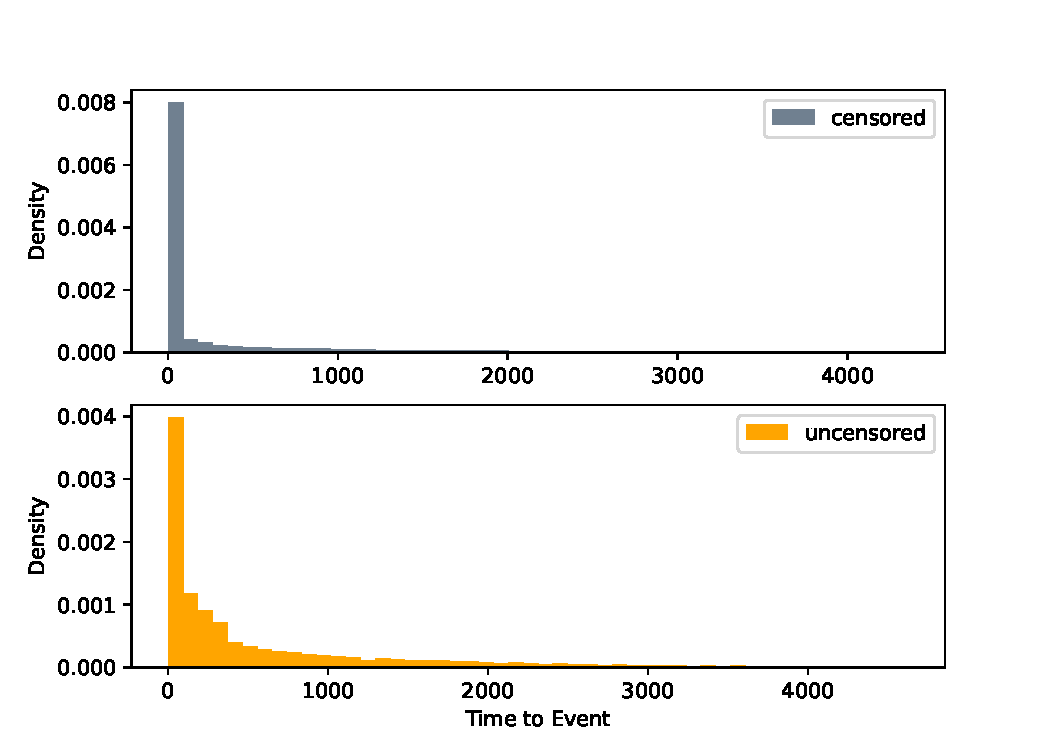
\includegraphics[width=0.5\textwidth]{cohort_hist.pdf}
  \caption{Cohort-wise Histogram}
  \label{fig:cohort_hist}
\end{figure}

\subsection{\label{censoring}Data Standardization}
Patients are randomly distributed into train, test and validation pools. Columns with zero variance in the training data are discarded from all three datasets - train, test and validation. Across each pool, their survival time is discretized into $q=15$ buckets or time intervals. For example, a patient whose survival time belongs to the $j^{th}$ bucket has experienced the event (or been censored) between the time interval $[q_j, q_{j+1})\ \forall j \in [1,2,\cdots,m]$.\\

For the time-invariant version, simple pipelines for imputation and scaling are carried out. For the time-varying version, the process is slightly more involved. First, a patient-level cumulative time difference column is introduced, to keep track of when medications or test were administered - for every patient, this column starts with 0. Next, a null mask $\mathcal{M}$ is created.


\section{\label{metrics}Evaluation Metrics}
As survival analysis differs from ordinary linear regression in the aspect that not all the survival times are known (right-censoring), there is merit in reviewing the evaluation metrics for this task. The two metrics used in the experimental setup are the time-dependent concordance index (in favour of the regular concordance index) and the Brier score (along with its aggregated version, the integrated Brier score).

\subsection{\label{tdci}Time-Dependent Concordance Index ($td$-concordance index)}
The C-index, often referred to as ``Harrell's C-Index'' or simply as the C-statistic is a measure of the discriminative capacity of a model. In essence, it is the generalization of the ROC (Receiver Operator Characteristic) curve - AUC in a survival analysis setting <Rephrase??> \cite{Uno_Cai_Pencina_D’Agostino_Wei_2011} \cite{pysurv}. The formula for the c-index is given as
%\[
%C-index = \frac{\sum_{i,j} \mathds{1}_{T_j < T_i}\cdot \mathds{1}_{\eta_j > \eta_i}\cdot d_j}{\sum_{i,j} \mathds{1}_{T_j < T_i}\cdot d_j}
%\]
\[
c = \frac{1}{|\mathcal{E}|}\sum_{i:C_i = 1}\sum_{T_j > T_i} \mathds{1}_{\eta_j > \eta_i}
\]
where $\eta_i$ denotes the predicted survival time for subject $i$. As c-index is rank-based index, it can be substituted with the survival probability of subject $i$ as well. $|\mathcal{E}|$ is the number of pairs that \textit{can} be compared.\\

It can be interpreted as the fraction of all pairs of subjects whose predicted survival times are correctly ordered among all subjects that can actually be ordered \cite{Pinto_Carvalho_Vinga_2015}. A pair $(i,j)$ is considered `comparable' if the one with the lower observed time is uncensored, that is, when $T_i <T_j$, then $d_i=1$. A pair is considered `concordant' when the model predicts a higher risk for the patient with a lower survival time. Thus, it follows that
\[ c-index = 
\begin{cases}
    1.0, & \text{perfect concordance}, \\
    0.5, & \text{equivalent to random classification}, \\
    0.0, & \text{perfect anti-concordance}.
\end{cases}
\]

There are limitations with the traditional c-index as highlighted by \cite{Hartman_Kim_He_Kalbfleisch_2023}, an important one being the assumption that the risk scores do not change over time. \cite{Heagerty_Zheng_2005} propose a time-dependent concordance index which essentially takes a weighted average of time-specific C-index values across the entire time scale.

\subsection{\label{ibs}Brier Score}

Contrasting the discriminatory power of the C-index, the Brier score provides a measure of how well the model is calibrated. It represents the distance between observed and predicted survival probability - hence 0 is the most desirable value. Given the data, $\mathcal{D}$, a set of tuples $\{(x_i , t_i , d_i)\}_{i=1}^{N}$ and the predicted survival function $\hat{S}(t, x_i),\ \forall t \in \mathbb{R^{+}}$, the Brier score (without right-censored observations) assumes a form similar to the mean-squared-error.
\[
BS(t) = \frac{1}{N}\sum^{N}_{i=1}(\mathbb{I}_{T_i>t}-\hat{S}(t, x_i))^2
\]

With the occurence of right-censored data, the formula needs to be adjusted by the inverse probability of censoring weights method <cite?>. Let $\hat{G}(t) = P[C>t]$ be the estimator of the conditional survival function of the censoring times calculated using the Kaplan-Meier method, where C is the censoring time.

\begin{gather*}
BS(t) = \frac{1}{N}\sum^{N}_{i=1}\Bigg(\frac{(0-\hat{S}(t,x_i))^2 \cdot \mathbb{I}_{T_i\le t, d_i = 1}}{\hat{G}(T_i)} +\\
\frac{(1-\hat{S}(t,x_i))^2 \cdot \mathbb{I}_{T_i > t}}{\hat{G}(t)} \Bigg)
\end{gather*}

An aggregated version of this score provides a simpler (albeit more reductive) summary of the calibration of a model.
\[
IBS(t_{max})= \int^{t_{max}}_{0} BS(t) dt
\]

\section{\label{exp}Experiments and Fits}
A series of experiments were conducted on this data from both a time-invariant and a time-varying perspective. The  survival distributions were examined with non-parametric fitters - Kaplan-Meier fitter and Nelson-Aalen fitter. A short write-up on these methods can be found in the Appendix \ref{appdx}. \\

Next, a range of parametric, semi-parametric, tree-based and neural network-based methods were applied to the data and their evaluation criteria noted. To establish confidence intervals on said criteria, fits were run multiple times - all time-invariant models apart from Cox Proportional Hazards model and Weibull Accelerated Failure Time model were run 20 times. The model allowing for time-varying data was run 10 times. Thus, distributions of their cindex and integrated Brier scores were generated. The details are listed in Table \ref{tab:eval}.\\

\begin{table*}[t]
  \centering
  \begin{tabular}{|p{4cm}|p{6cm}|p{2cm}|p{2cm}|}
     \hline
    \textbf{Model} & \textbf{HyperParameters} & \textbf{C-Index} & \textbf{IBS} \\
    \hline
    Cox Proportional Hazards & penalizer = 0.1, step\_size = 0.1 & 0.6808 & 0.1685\\
    \hline
    Weibull AFT & penalizer = 0.01  & 0.6804 & 0.1748\\
    \hline
    Random Survival Forest & n\_estimators=1000, min\_samples\_split=10, min\_samples\_leaf=15, n\_jobs=-1, random\_state=1234, oob\_score = True  & 0.6975 & 0.1956\\
    \hline
    PyCox (with Logistic Hazard loss function \cite{kvamme_continuous_2019}) & discretization=15, layers=[256,256],  batch\_norm=True, dropout=0.5, batch\_size=256, epochs=500 & 0.5974 & 0.1768\\
    \hline
    Deep Survival Machhines & k=6, distribution=LogNormal, learning\_rate=1e-3, layers=[100, 100] & 0.6441 & 0.2724\\
    \hline
    DeepSurv & batch\_size=256, num\_epochs=1000, learning\_rate=0.01, patience=50, hidden\_size=100, 
droutput\_rate = 0.1 & 0.4259 & - \\    
    \hline
    Time-Invariant Survival & clusters=1, discretizations = 15, hidden\_size = 25 , alpha = 0.05 , batch\_size=256, num\_epochs=400, learning\_rate=0.001, patience=20, dropout\_rate = 0.5, mc\_iter = 100 & - & - \\
    \hline
    Time-Variant Survival & discretizations = 15, hidden\_size = 25 , alpha = 0.01 , batch\_size=256, num\_epochs=100, learning\_rate=0.001, patience=20, dropout\_rate = 0.5, mc\_iter = 100  & - & - \\
    \hline
  \end{tabular}
  \caption{Evaluation metrics}
  \label{tab:eval}
\end{table*}


\section{\label{conc}Conclusions}
The architecture is sacrificing calibration for discriminatory power. The figures \ref{fig:cindex} and \ref{fig:ibs} showcase this situation.

\begin{figure*}[t]
  \centering
  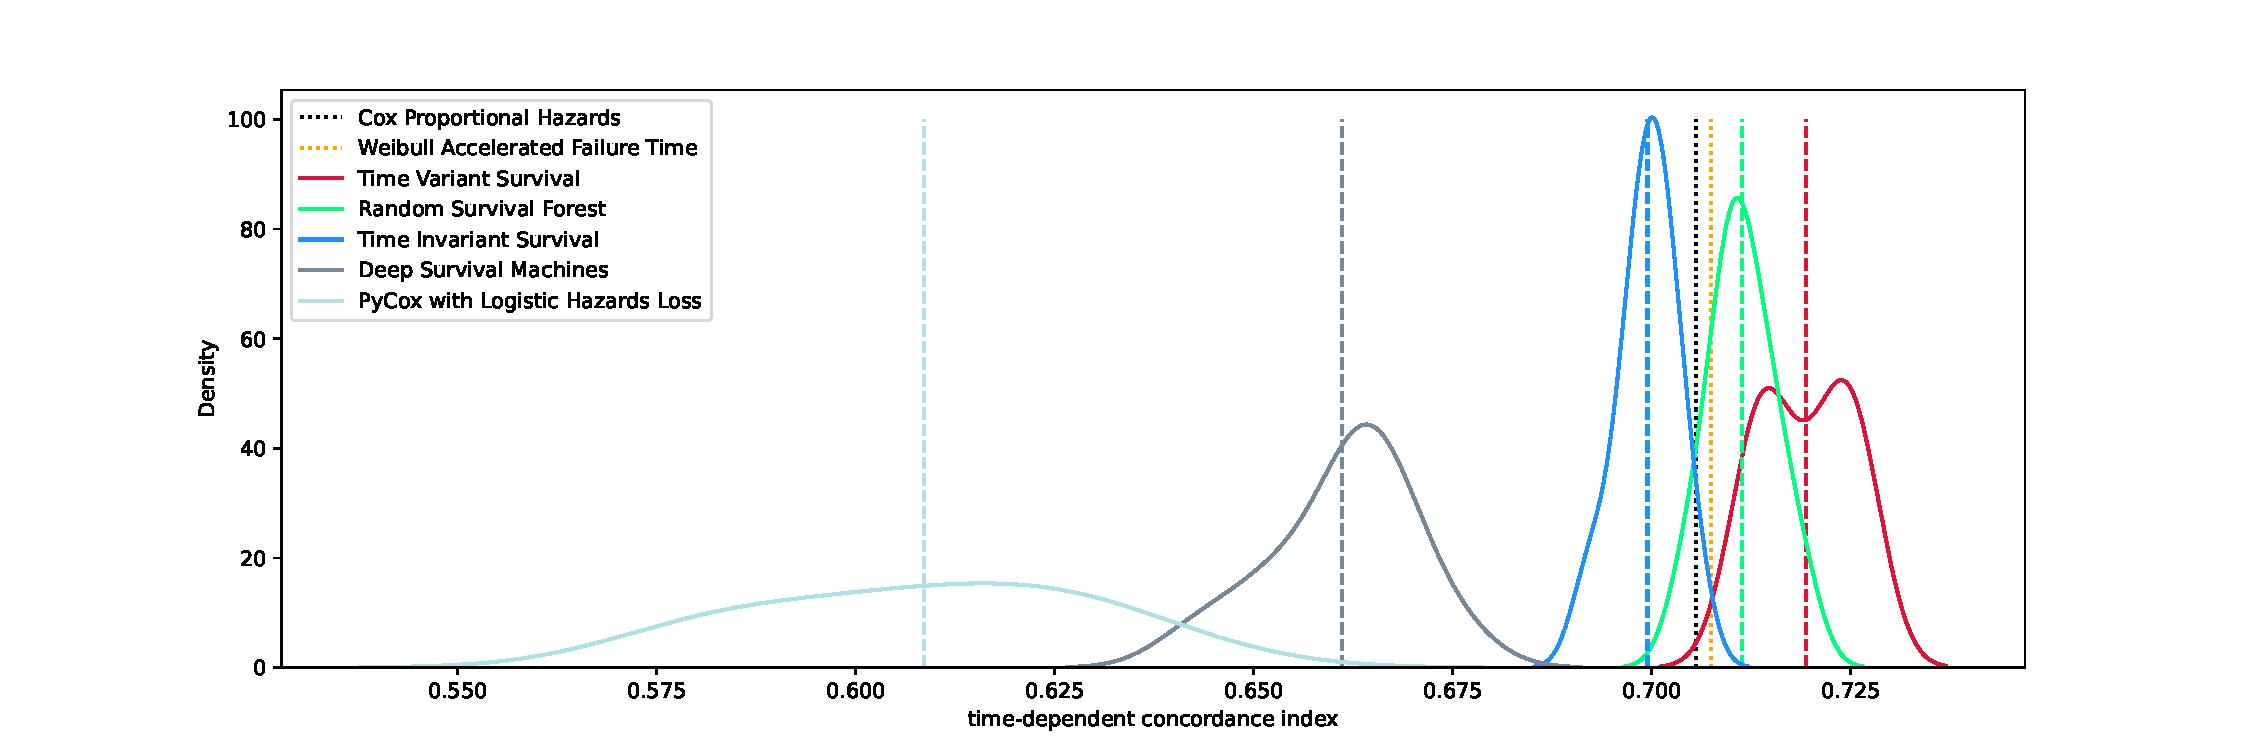
\includegraphics[width=\textwidth]{cindex_score_dist_plot.pdf}
  \caption{Distribution of C-index}
  \label{fig:cindex}
\end{figure*}


\begin{figure*}[t]
  \centering
  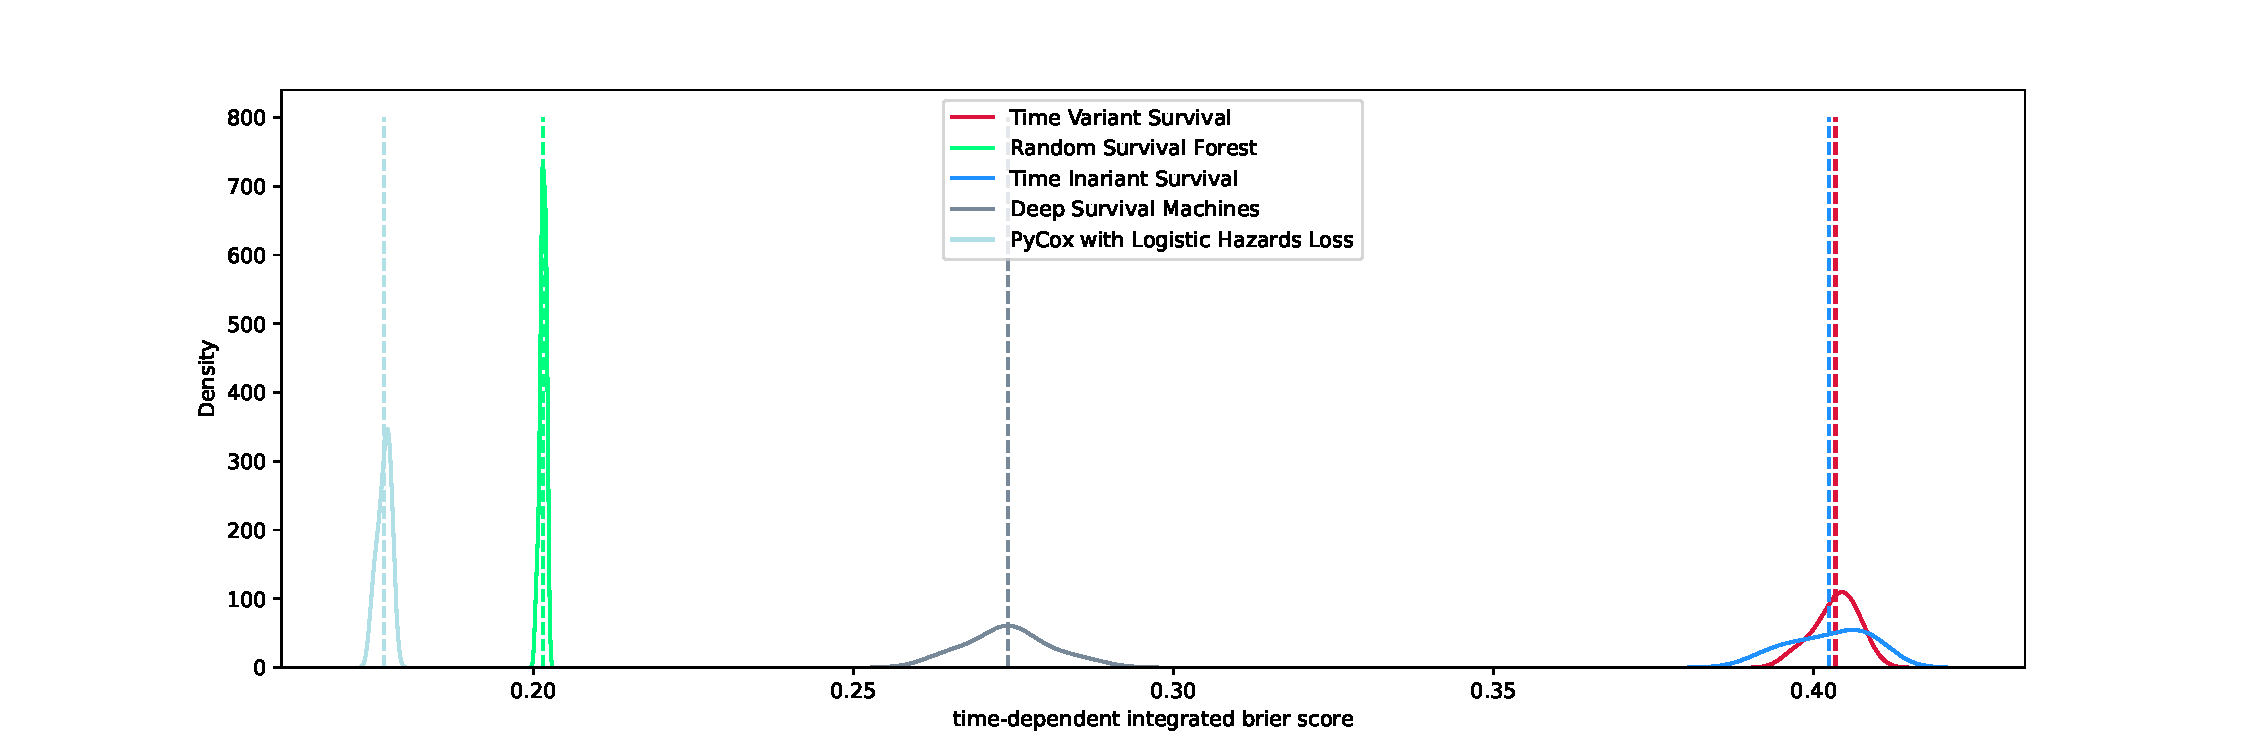
\includegraphics[width=\textwidth]{ibs_score_dist_plot.pdf}
  \caption{Distribution of IBS}
  \label{fig:ibs}
\end{figure*}

\section{\label{morework}Further Work}
Other neural network methods capable of temporal learning (forms of RNN) can be applied to this problem to see if the discriminative power can be increased.

\cite{*}

\bibliography{references}% Produces the bibliography via BibTeX.

\appendix

\section{\label{appdx}Appendix}

Some formal mathematical formulations of the methods used in this paper are elaborated in the following sections
\subsection{\label{non_param}Non-Parametric Fits}
The Kaplan Meier fitter

The Nelson Aalen

MLP

CNN

MC dropout

SHAP

\section{\label{perf}Performance Metrics}
Times of all the fitters.


\section{\label{perf}Performance Metrics}
All relevant code for this study can be found on \href{https://github.com/sourasen1011/UoE_Research_Project_2023/tree/dev}{sourasen1011/UoE\_Research\_Project\_2023/tree/dev}.
\end{document}
%
% ****** End of file apssamp.tex ******
